Chương này trình bày lý do chọn đề tài -- sự cần thiết đo độ tương tự
giữa các chương trình máy tính -- cùng mục tiêu nghiên cứu, đối tượng và phạm
vi nghiên cứu, cũng như những nghiên cứu có liên quan đến đề tài.

\section{Lý do chọn đề tài}

Hiện nay, ngành Công nghệ thông tin đang có xu hướng phát triển mạnh
mẽ và học trực tuyến ngày càng trở nên phổ biến. Một số chương trình
đào tạo trực tuyến nổi tiếng như
\href{https://www.coursera.org/course/saas}{Massive Open Online
  Courses (MOOC)} \cite{mooc}, \href{https://www.edx.org/}{edX}
\cite{edx}, \href{https://www.coursera.org/}{Coursera}
\cite{coursera}, \href{http://www.udacity.com/}{Udacity}
\cite{Udacity} (Hình \ref{fig:progarming-online}) ngày càng có nhiều người tham gia. Ngoài ra, một số
chương trình hỗ trợ rèn luyện kỹ năng lập trình trực tuyến như
\href{https://www.pexforfun.com/}{Pex4Fun} \cite{Pex4Fun} hay
\href{https://www.microsoft.com/en-us/research/project/code-hunt/}{Code
  Hunt} \cite{CodeHunt} cũng thu hút nhiều sự quan tâm của nhiều
người. 

\begin{figure}[h]
	\centering
	
\includegraphics[scale=.4]{topMOOC.png}
	\caption{Một số chương trình đào tạo trực tuyến nổi tiếng}
	\label{fig:progarming-online}		
\end{figure}

Một trong những thách thức của việc đào tạo lập trình trực tuyến là
làm sao cho phép tổ chức những lớp học có quy mô lớn, trong khi đó vẫn
đảm bảo chất lượng đào tạo. Thông thường, những khóa học trực tuyến
phổ biến có rất nhiều học viên tham gia, hàng trăm thậm chí hàng ngàn
người, nhưng số người phụ trách giảng dạy không nhiều. Sự hạn chế về
số người phụ trách này có ảnh hưởng rất nhiều đến chất lượng đào
tạo. Về phía người giảng dạy, để xếp hạng học viên hay cung cấp những
phản hồi đối với từng lời giải của học viên đòi hỏi họ phải đọc hiểu
toàn bộ mã lệnh do học viên viết. Công việc này dường như quá nặng
nhọc nhưng không thể bỏ qua hoặc trì hoãn vì như vậy sẽ không thể bắt
kịp tiến độ của học viên. Ngoài ra, về phía học viên, họ đến từ rất
nhiều nơi trên thế giới nên thời gian học cũng khác nhau. Những lúc họ
gặp khó khăn trong việc viết mã chương trình, họ có thể tìm kiếm sự
trợ giúp từ bạn bè hoặc những người có kinh nghiệm, từ người dạy. Tuy
nhiên, không phải lúc nào cũng có người này cũng có bên cạnh để giúp
đỡ cho họ, ảnh minh họa Hình \ref{fig:Retry}. 

\begin{figure}[h]
	\centering
	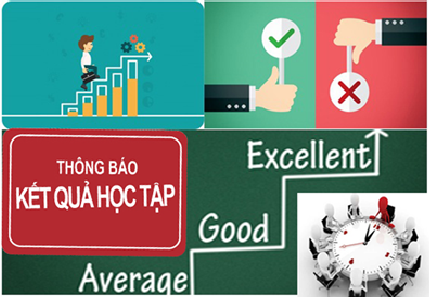
\includegraphics[scale=.8]{Retry.png}
	\caption{Những khó khăn của người dạy và người học}
	\label{fig:Retry}		
\end{figure}

Thách thức trên có thể giải quyết nếu có được công cụ tự động hóa việc
so sánh giải pháp của học viên đưa ra so với giải pháp của giáo viên
xem chúng có tương đương không, hay tương tự nhau ở mức độ nào. Sự
tương đương giữa hai chương trình được hiểu theo nghĩa chúng cho ra
cùng kết quả nếu nhận vào cùng dữ liệu. Việc chuyển đổi từ dữ liệu vào
thành dữ liệu ra của một chương trình có thể xem là \emph{hành vi} của
nó. Công cụ này có thể giúp người dạy đánh giá xếp hạng giải pháp của
học viên dựa vào giải pháp của mình. Ngoài ra, công cụ còn có thể giúp
đánh giá được người học có tiến bộ không, giúp đưa ra những gợi ý lập
trình cho học viên,\dots

Chúng tôi nhận thấy vấn đề cốt lõi để xây dựng công cụ này là làm sao
đo được độ tương tự về hành vi giữa hai chương trình. Đó là lý do tôi chọn đề tài \emph{``Độ tương tự hành vi của chương trình và thực nghiệm''}. Đề tài này  sẽ làm rõ hành vi của chương trình, độ tương tự về hành vi của chương trình và một số phương pháp đo độ tương tự về hành vi.

\section{Đối tượng, phạm vi, phương pháp nghiên cứu}
\subsection{Mục tiêu nghiên cứu}

Mục tiêu nghiên cứu chính của luận văn là tìm cách đánh giá độ tương tự về hành vi giữa hai chương trình máy tính. Nó được cụ thể hóa thành những mục tiêu sau:
\begin{itemize}
\item Tìm hiểu sự tương tự hành vi của chương trình;
\item Tìm hiểu kỹ thuật, công cụ sinh test case tự động và áp dụng để
  đo độ tương tự về hành vi;
\item Tìm cách kết hợp các kỹ thuật đo với nhau;
\item Đánh giá kết quả thực nghiệm.
\end{itemize}

\subsection{Đối tượng, phạm vi nghiên cứu}

\subsubsection*{Đối tượng nghiên cứu}

Đối tượng nghiên cứu chính trong luận văn này gồm:
\begin{itemize}
\item Kỹ thuật sinh Test Case
\item Các kỹ thuật đo độ tương tự hành vi
\item Ứng dụng của các kỹ thuật đo độ tương tự hành vi
\end{itemize}
	
\subsubsection*{Phạm vi nghiên cứu}
\begin{itemize}
\item Đo độ tương tự hành vi dựa vào Test Case
\item Thực nghiệm, đánh giá trên các chương trình C\#
\end{itemize}


\subsection{Phương pháp nghiên cứu, thực nghiệm}
\subsubsection*{Nghiên cứu lý thuyết}
\begin{itemize}
\item Độ tương tự hành vi
\item Một số kỹ thuật sinh Test Case tự động
\item Kỹ thuật đo độ tương tự hành vi dựa trên Test Case
\item So sánh, kết hợp các phép đo độ tương tự hành vi
\end{itemize}
		
\subsubsection*{Thực nghiệm}
\begin{itemize}
\item Tiến hành cài đặt các kỹ thuật đo độ tương tự hành vi
\item Thực nghiệm trên dữ liệu thực của CodeHunt, và một số dữ liệu thử khác
\item Phân tích, đánh giá dựa trên kết quả thực nghiệm
\end{itemize}


\section{Những nghiên cứu có liên quan}

Đề tài này liên quan đến những nghiên cứu về xếp hạng tự động, sự
tương đương giữa hai chương trình, phát hiện đạo code.

\subsection*{Xếp hạng tự động}
	
Trong bài báo \cite{alur2013automated} nhóm tác giả đề xuất một phương
pháp tự động so một automat hữu hạn đơn định chưa đúng của sinh viên
với automat hữu hạn đơn định của giáo viên dùng làm automat tham
chiếu. Cách tiếp cận này của các tác giả sử dụng các kỹ thuật đo sự
khác nhau về cả cú pháp và ngữ nghĩa giữa hai automat. Sự khác biệt về
cú pháp được đo qua khoảng cách chỉnh sửa (\emph{syntactic edit
  distance}) và sự khác biệt về ngữ nghĩa được đo dựa trên các
câu vào được đoán nhận bởi automat (\emph{accepted string
  inputs}). Mặc dù cách tiếp cận của nhóm tác giả bài báo và tác giả
luận văn đều sử dụng khái niệm về độ tương tự về ngữ nghĩa, cách tiếp
cận của bài báo dùng cho automat hữu hạn đơn định trong khi các độ đo
trong luận văn dùng cho các chương trình máy tính.

Một bài báo khác liên quan đến chủ đề này là \cite{singh2013automated}. Trong đó, nhóm tác giả đề xuất phương pháp tự động
xác định số sửa lỗi tối thiểu cần thực hiện trên chương trình của sinh viên (chưa đúng) sao cho khớp với giải pháp tham chiếu của giáo viên. Cách tiếp cận này cung cấp cách sử lỗi thông qua việc tính khoảng cách cú pháp tối thiểu (\emph{minimal syntactic distance}) giữa chương trình sai với chương trình tham chiếu, trong khi đó luận văn tập trung vào đo độ tương tự về ngữ nghĩa của hai chương trình dựa vào các hành vi vào/ra. Các độ đo trong luận văn có thể nhận biết độ tương tự giữa các chương trình có cấu trúc cú pháp khác nhau.

Ngoài ra, trước những nghiên cứu vừa nêu được đưa ra, trong bài báo
\cite{wang2007semantic}, tác giả đề xuất một giải pháp đo độ tương tự
về ngữ nghĩa của hai chương trình thông qua việc chuyển đổi chương
trình của học viên và chương trình tham chiếu của giáo viên về một
dạng chung nhưng không thay đổi ngữ nghĩa, đó là đồ thị phụ thuộc
(\emph{dependence graphs}), rồi tiến hành so sánh hai đồ thị để tính
toán sự tương đồng. Thay vì so sánh các đồ thị, cách tiếp cận của đề
tài này là so sánh các cặp đầu vào, đầu ra của các chương trình để
tính toán các điểm tương đồng về hành vi.
	
\subsection*{Kiểm tra sự tương đương giữa hai chương trình}

Có một số phương pháp kiểm tra sự tương đương về ngữ nghĩa/hành vi của
các chương trình bằng cách sử dụng đồ thị phụ thuộc
\cite{bates1993incremental,binkley1992using}, sự phụ thuộc giữa giá
trị đầu vào và đầu ra \cite{jackson1994semantic}. Tất cả các cách tiếp
cận để kiểm tra độ tương đương này đều trả về giá trị logic
đúng/sai. Tuy nhiên, ngoài việc kiểm tra sự tương đương, giải pháp
trong luận văn này còn có thể đo được độ tương tự giữa hai chương
trình.

Phương pháp tự động xác định những đoạn mã tương đương nhau về chức
năng thông qua các phép thử ngẫu nhiên
\cite{jiang2009automatic}. Cách tiếp cận này xem xét hai đoạn mã có
tương đương nhau hay không thông qua giá trị đầu vào và đầu ra, không
quan tâm đến cấu trúc và cú pháp của chúng. Độ đo RS trong luận văn này cũng tương tự với cách tiếp cận trong bài báo. Tuy nhiên, luận văn này các đưa ra hai phương pháp đo khác, dựa trên kỹ thuật thực thi biểu trưng chương trình DSE (\emph{Dynamic Symbolic Execution}).
	
% \subsection*{Phản hồi dựa trên trường hợp các thử nghiệm}

% Phương pháp tự động phân loại chương trình, bài tập đơn giản
% \cite{hext1969automatic}, cách tiếp cận của phương pháp này là so sánh
% dữ liệu được tạo ra trong quá trình thực thi chương trình với dữ liệu
% đã lưu trữ trước đó.
	
% Phương pháp phân loại chương trình của sinh viên sử dụng ASSYST
% \cite{jackson1997grading}, tác giả đề xuất cách tiếp cận đó là tự động
% kiểm tra tính chính xác của chương trình và kiểu lập trình như mô đun,
% độ phức tạp và hiệu quả.
	
% Pex4Fun sử dụng DSE để tạo ra các giá trị đầu vào thử nghiệm cho các
% chương trình và các chương trình khi thực thi các giá trị này sẽ cho
% ra các giá trị đầu ra khác nhau.
	
\subsection*{Phát hiện đạo code}

Những nhà nghiên cứu đã đề xuất các tiếp cận tính cho việc tính toán
độ tương tự giữa các biến thể của các đoạn mã lệnh để tự động nhận
diện đạo code, như sử dụng cây cú pháp trừu tượng
\cite{baxter1998clone}, đồ thị phụ thuộc của chương trình
\cite{komondoor2001using}, các độ đo dựa trên các đơn vị cú pháp (như
các lớp, hàm) \cite{dang2012xiao} \cite{merlo2004linear}. Các tiếp cận
này tính toán độ tương tự bằng cách phân tích tĩnh các đoạn mã lệnh
còn cách tiếp cận trong luận văn về việc tính độ tương tự bằng cách
thực thi chương trình để sinh ra các cặp dữ liệu vào/ra, làm cơ sở để
tính toán.
	
\section*{Tổng kết chương}

Ngày nay, những chương trình đào tạo trực tuyến ngày càng có nhiều
người tham gia, có thể lên đến hàng trăm, thậm chí hàng ngàn người mỗi
lớp. Thách thức quan trọng là làm sao tổ chức được các lớp có quy mô
lớn nhưng vẫn đảm bảo chất lượng giáo dục trong điều kiện số lượng
người tham gia giảng dạy cho mỗi lớp có hạn chế. Phương pháp đo độ
tương tự về hành vi giữa hai chương trình máy tính làm cơ sở để xây
dựng công cụ tự động hóa nhằm giảm thiểu công sức người dạy trong việc
đánh giá xếp hạng kết quả học tập của học viên cũng như đưa ra những
gợi ý hỗ trợ cho người học trong quá trình viết chương trình.
Chương \ref{chap:intro} cho thấy sự cần thiết của đề tài cũng như đối tượng, phạm vi và phương pháp nghiên cứu. Ngoài ra, chương này còn trình bày một số nghiên cứu có liên quan về việc xếp hạng tự động, kiểm tra sự tương đương, phát hiện đạo code.

Phần còn lại của luận văn được tổ chức thành hai chương. Chương
\ref{chap:method} làm rõ về hành vi của chương trình cùng những phương
pháp đo độ tương tự về hành vi. Chương \ref{chap:results} trình bày
kết quả thực nghiệm cùng một số vấn đề liên quan.





%%% Local Variables:
%%% mode: latex
%%% TeX-master: "Main"
%%% End:
